\problemname{Marsmeddelanden}
I filmen \emph{The Martian} blir astronaut Mark Watney fast på Mars. Jorden kommunicerar med Mark genom att rotera
kameran på en gammal rymdsond.

Sonden pekar på en hexadecimal siffra, d.v.s. \texttt{0-9} eller \texttt{a-f}, och Mark bildar sedan bokstäver
och andra tecken genom att konvertera par av dessa siffror enligt teckenkodningen ASCII. För att tyda
vilken siffra sonden pekar på har han delat in en hel cirkel om 360 grader i 16 lika stora bitar om 22.5 grader
vardera.

\begin{figure}[h!]
  \begin{center}
    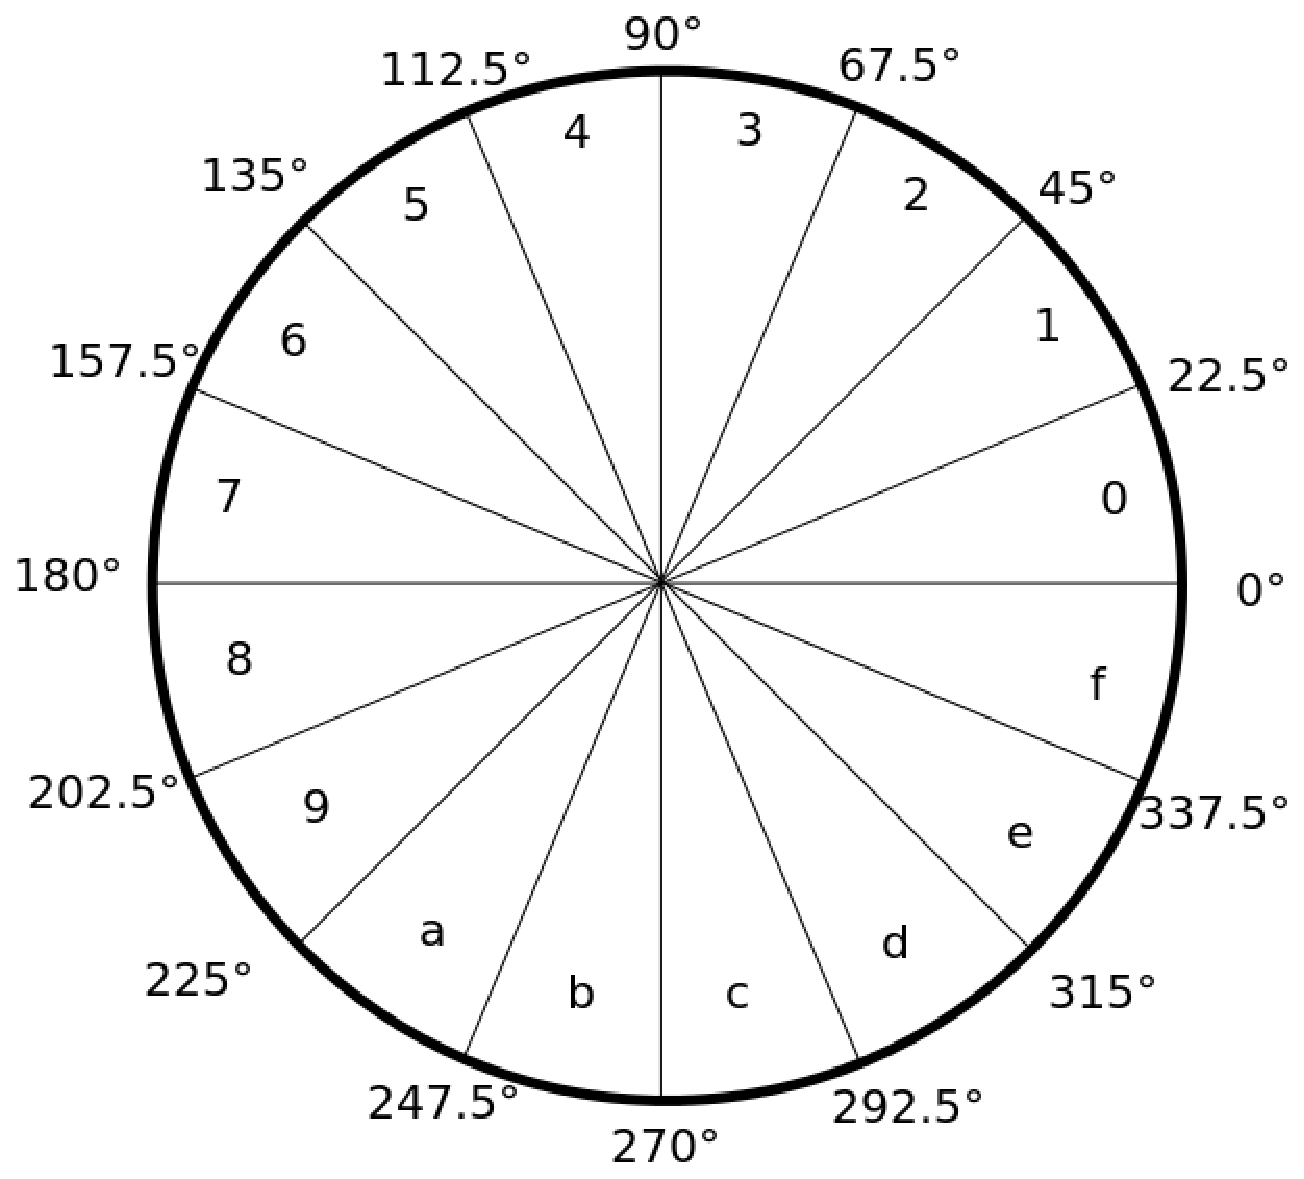
\includegraphics[width=0.3\textwidth]{angles.eps}
  \end{center}
\end{figure}

Som ett exempel representerar vinkelparet $(100^{\circ}, 30^{\circ})$ det hexadecimala talet 41, vilket är talet $65$ decimalt.
Enligt ASCII representerar detta tecknet \texttt{A}.

Nu har Mark tröttnat lite på att skriva ner dessa siffror manuellt, och har bett dig om hjälp med att avkoda meddelandet
som han får. Du kommer få sekvensen av de vinklar som sonden pekar på, och ska skriva ut meddelandet.

\section*{Input}
Den första raden innehåller ett heltal $2 \le N \le 50\,000$, antalet vinklar du ska läsa in. $N$ garanteras vara ett jämnt tal.
De nästa $N$ raderna innehåller vinklarna, en vinkel per rad. Vinkeln ges som ett flyttal i grader i intervallet $[0, 360)$.
Det är garanterat att sonden aldrig pekar på någon vinkel som ligger precis mellan två hexadecimala siffror.
Det är också garanterat att under avkodningen till ASCII kommer enbart tecken med decimala värden \texttt{32-126} ges.

\section*{Output}
Du ska skriva ut en enda rad med de tecken som meddelandet avkodas till.

\section*{Poängsättning}
Din lösning kommer att testas på en mängd testfallsgrupper. För att få poäng för en grupp så måste du klara alla testfall i gruppen.

\begin{tabular}{| l | l | l |}
	\hline
	Grupp & Poängvärde & Begränsningar\\ \hline
  1     & 46         & alla vinklar är heltal \\ \hline
  2     & 54         & \\ \hline
\end{tabular}
